\subsection{Training ViT}
Results visible in next pages were obtained using ViT model trained with the hyperparameters visible on \prettyref{lst:vit-hyperparameters}.

\newenvironment{longlistingI}{\captionsetup{type=listing, width=0.8\textwidth}}{}
\begin{longlistingI}
    \pythoncode{listings/vit_hyperparameters.py}
    \caption{ViT model initialization}
    \label{lst:vit-hyperparameters}
\end{longlistingI}
\vspace{12pt}

For the training phase, 90,000 samples were generated, comprising 10,000 samples for different number of elements ranging from 1 to 9. 
90\% of the samples were utilized in the training step, while the remaining 10\% were allocated for the validation. 
The Adam optimizer was employed with a learning rate of 0.0001, and Binary Cross Entropy loss was used because multi-label classification reduces to multiple binary classification problems.

The model was trained for 10 epochs, with a batch size of 128. 
Loss through epochs can be seen on \prettyref{fig:vit-loss}. 
Training loss was averaged over all mini batches in epoch, which is why it is generally larger than validation loss, which was calculated after the epoch. 

After training, the ROC (Receiver Operating Characteristics) curve over 5000 random samples was calculated to assess the model's performance. 
The ROC curve is a plot of recall (sensitivity) against $1-\text{specificity}$ \cite{rocCurve}.
Recall, also known as the TPR (True Positive Rate) measures the ability of a model to capture all the relevant instances and is defined as \(\frac{\text{TP}}{\text{TP} + \text{FN}}\) (look \prettyref{tab:classification_matrix} for abbreviations).
$1-\text{specificity}$, or FPR (False Positive Rate) is defined as \(1 - \frac{\text{TN}}{\text{TN} + \text{FP}} = \frac{\text{FP}}{\text{TN} + \text{FP}}\) and says what proportion of actual positive instances were are incorrectly identified as negative.
When the threshold for positive classification, e.g., 0.5, is lowered, the number of positive classifications increases, resulting in an increase of both TPR and FPR. 
However, lowering the threshold will lead to an increase in false positives, possibly greater than true positives, causing the \(\frac{\text{TPR}}{\text{FPR}}\) ratio to decrease.

In general, better classifiers should have a greater area under the ROC curve, known as AUC (Area Under the Curve). 
The ROCs and AUCs were calculated using the best weights of the trained model and are visible in \prettyref{fig:roc-auc}.

\begin{figure}[htbp!]
  \centering
  \includesvg[width=0.8\textwidth]{img/vit_loss.svg}
  \caption{Loss in each training epoch}
  \label{fig:vit-loss}
\end{figure}

\begin{figure}[htbp!]
  \centering
  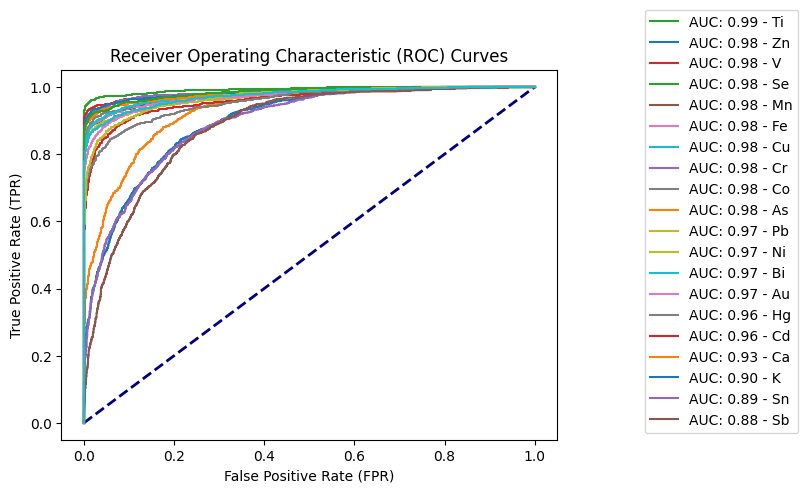
\includegraphics[width=1\textwidth]{img/roc_auc.png}
  \caption{ROC and AUC of each trained element}
  \label{fig:roc-auc}
\end{figure}

ROC of a few elements, namely Ca, K, Sn, and Sb, seems to differ significantly from the rest. 
The energies of their spectral lines are as follows: 3.692, 3.314, 3.444, and 3.604 [keV]. 
As one can see, these values are quite close to each other, and the elements do not have any other lines defined in the code that could help differentiate between elements.
In that case model could be improved by using more accurate theoretical element spectra. 

Besides ROC, a few metrics were evaluated for different number of elements in spectra, namely: accuracy, precision, recall and f1 score. 
Precision measures the accuracy of the positive predictions and is evaluated as $\frac{TP}{FP+TP}$ .
f1 score is popular metric that unifies precision and recall under one metric evaluated as a harmonic mean  $2\times\frac{precision \times recall}{precision + recall}$.
The evaluation was conducted on 1000 random samples within each category and is visible on \prettyref{fig:vit-metrics}.

Based on the precision histogram, it can be concluded that the count of false positives grows rapidly with an increase in elements in the spectrum. It is hard to determine how this issue may be mitigated; perhaps the best course of action is to compare results with another method. 
Besides attempts to improve the existing model, hyperparameters or training process, it may be worthwhile to try training separate classifiers for each element and assess whether such an approach could yield better results.

\begin{figure}[htbp!]
  \centering
  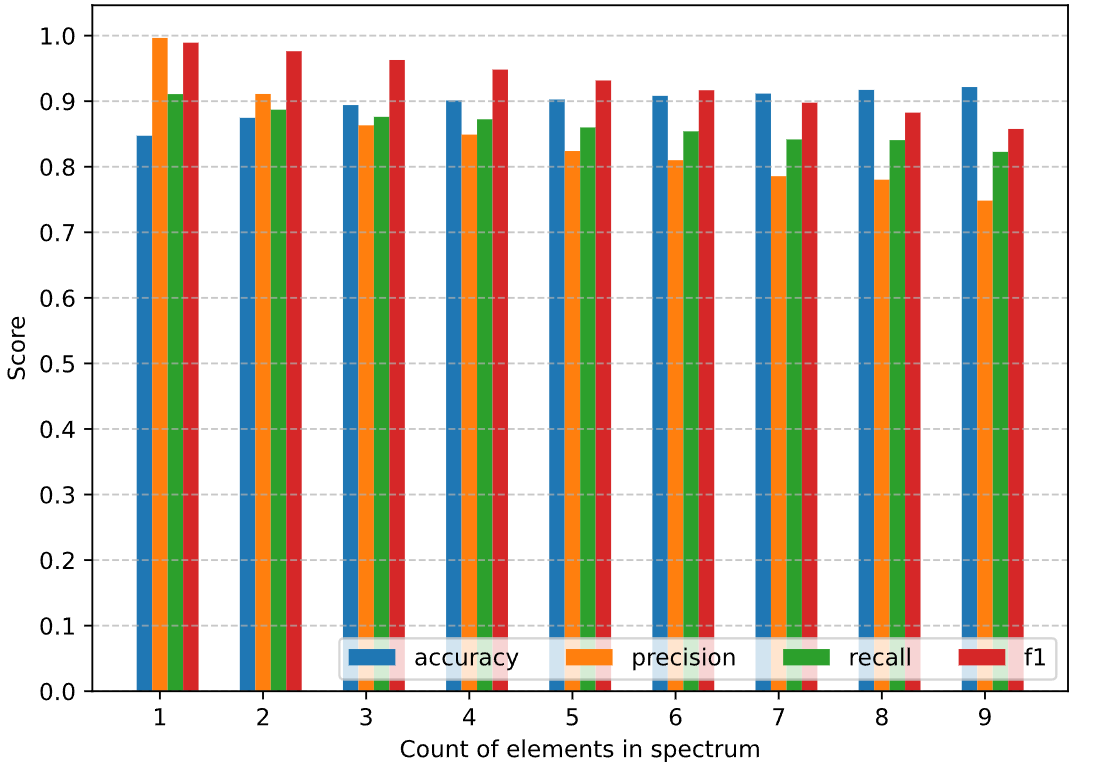
\includegraphics[width=0.8\textwidth]{img/metrics.png}
  \caption{Metrics for different number of elements in spectrum}
  \label{fig:vit-metrics}
\end{figure}

\begin{table}[htbp!]
  \centering
  \begin{tabular}{|c|c|c|}
    \hline
    & \textbf{Real Positive} & \textbf{Real Negative} \\
    \hline
    \textbf{Predicted Positive} & TP (True Positive) & FP (False Positive) \\
    \hline
    \textbf{Predicted Negative} & FN (False Negative) & TN (True Negative)  \\
    \hline
  \end{tabular}
  \caption{Classification matrix}
  \label{tab:classification_matrix}
\end{table}

